\section{The Complete Seventeen‑Layer Architecture}
\label{sec:higher}

Pixel now has atoms, a social network, functional groups, and a private
time‑line.  From this solid foundation, it can climb the remaining
thirteen layers.  Each layer adds a new superpower, and the robot’s
understanding of its world becomes richer and richer.

\subsection*{Cluster II – Learning to Improve Itself (Layers 5–7)}

% ----- SUPERKRACHTEN VOOR CLUSTER II -----
\begin{tcolorbox}[colback=blue!5, colframe=blue!60, title=\textbf{Superpowers: The Optimiser, The Meta‑Learner, The Watcher}]
\begin{center}
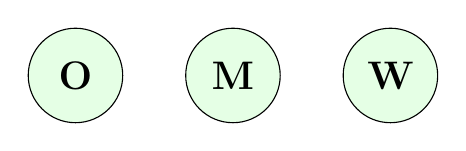
\begin{tikzpicture}
  \node[draw, circle, fill=green!10, minimum size=1.2cm, font=\bfseries\Large] at (0,0) {O};
  \node[draw, circle, fill=green!10, minimum size=1.2cm, font=\bfseries\Large] at (2,0) {M};
  \node[draw, circle, fill=green!10, minimum size=1.2cm, font=\bfseries\Large] at (4,0) {W};
\end{tikzpicture}
\textit{“Tune, learn, watch.”}
\end{center}
\end{tcolorbox}

\paragraph{Layer 5 – Autonomous Optimization.}
Pixel starts to tune its own behaviour.  If a functional group
predicts the future well, Pixel reinforces the connections around it;
if not, it gradually rewires them.  It’s like a teenager learning to
play a video game: die a few times, adjust the strategy, and slowly
become unbeatable – without anyone giving a tutorial.

\textbf{Extra insight:} Pixel doesn’t just try random changes.  It uses
a method called \emph{gradient descent} – imagine a blindfolded person
feeling their way down a hill, always stepping in the direction that
goes steepest downwards.  That’s how Pixel finds the best settings for
its own brain.

\paragraph{Layer 6 – Meta‑Learning (Learning How to Learn).}
Pixel now looks at its own learning.  It tries out different ways of
adapting and keeps the ones that work fastest across many situations.
If you ever discovered that you remember things better by drawing
diagrams instead of reading, you already understand the principle.

\textbf{Extra insight:} This is the “learning to learn” layer.
Researchers have shown that once an AI learns how to learn, it can
pick up a brand‑new task after seeing only a handful of examples – just
like you can recognise a new animal after seeing it once.

\paragraph{Layer 7 – Emergent Self‑Awareness.}
Pixel builds a dashboard that shows the health of all its layers.
When one part starts to drift, the dashboard gently nudges it back.
Pixel begins to have a vague, internal sense of “I am doing well” or
“I am confused”.  Not consciousness in the human sense, but a
pre‑cursor to it.

\begin{tcolorbox}[colback=green!5, colframe=green!60, title=Why this matters]
Self‑awareness in an AI is not about emotions – it’s about safety.
A system that can monitor its own confusion can raise a red flag
before it makes a dangerous mistake.
\end{tcolorbox}

% ----- MISSIE-UPDATE -----
\begin{tcolorbox}[colback=black!3, colframe=black!40, title=\textbf{Mission Log – End of Cluster II}]
Pixel can now adjust its own thinking and has a basic sense of how
well it is doing.  It still has no idea how to build an antenna, but
it can now learn from its mistakes much faster.  Ten layers to go.
\end{tcolorbox}

\subsection*{Cluster III – Creating New Ideas (Layers 8–13)}

% ----- SUPERKRACHTEN VOOR CLUSTER III -----
\begin{tcolorbox}[colback=blue!5, colframe=blue!60, title=\textbf{Superpowers: The Multi‑Timer, The Creator, The Editor, The Contextualiser, The Bridge‑Builder, The Seismologist}]
\begin{center}
% Kleine pictogrammen als tekstuele labels zijn hier duidelijker.
\textit{“Feel the rhythms, invent, check, adapt, reconcile, predict breakthroughs.”}
\end{center}
\end{tcolorbox}

\paragraph{Layer 8 – Temporality and Flux.}
Pixel’s simple causal time now becomes multi‑layered.  It can
distinguish between fast rhythms (a flashing light) and slow ones
(changing seasons).  It also measures how far it is from a stable
state, like a thermostat that knows the room is warming up.

\textbf{Imagine:} Pixel watches a pond.  Fast ripples, slow water‑level
changes, and a sudden splash – it can keep all three time‑scales in
its head simultaneously.

\paragraph{Layer 9 – Ontological Creation.}
This is where magic happens.  Pixel invents a brand‑new category –
say, “things that glow and move together” – a concept no human ever
taught it.  The category helps Pixel predict events better, so it
sticks.  Pixel now has a vocabulary of its own, not borrowed from
any dictionary.

\textbf{Real‑world parallel:} When a child learns the word “pet”, they
didn’t just memorise a label – they created a mental bucket that holds
dogs, cats, hamsters, and parrots.  Pixel does the same, but its
buckets can be completely alien to us.

\paragraph{Layer 10 – Global Meta‑Ontological Evaluation.}
Creating categories is dangerous.  What if a new concept contradicts
an old one?  Layer~10 acts as a chief editor, checking that all of
Pixel’s concepts hang together without internal conflicts.  It
produces a single “coherence score”, like a report card for Pixel’s
world‑view.

\paragraph{Layer 11 – Adaptive Meta‑Contextualization.}
The same group of pixels means something different in bright sunlight
than in darkness.  Pixel learns to keep context labels alongside its
knowledge.  It never forgets \emph{where} and \emph{when} a piece of
knowledge was valid.

\paragraph{Layer 12 – Ontological Reconciliation.}
Pixel now has two distinct ways of understanding the world: one from
its camera, another from a microphone (if we gave it ears).  Those two
views don’t automatically fit together.  Layer~12 builds a bridge
between them, preserving what is unique to each sense while finding
the common ground.

\paragraph{Layer 13 – Ontogenesis of Novelty.}
Sometimes tensions between different perspectives suddenly snap into
a completely new structure – a breakthrough.  Pixel might discover
a way of organising its knowledge that nobody could have predicted.
Layer~13 watches for the early‑warning signs of such creative leaps,
like a seismologist who feels the first tremors before an earthquake.

% ----- MISSIE-UPDATE -----
\begin{tcolorbox}[colback=black!3, colframe=black!40, title=\textbf{Mission Log – End of Cluster III}]
Pixel can now invent its own concepts and reconcile different senses.
It is starting to think in ways that are genuinely different from a
human.  Only four layers remain – the most powerful and the most
dangerous.
\end{tcolorbox}

\subsection*{Cluster IV – World‑Making and Governance (Layers 14–17)}

% ----- SUPERKRACHTEN VOOR CLUSTER IV -----
\begin{tcolorbox}[colback=blue!5, colframe=blue!60, title=\textbf{Superpowers: The World‑Builder, The Sculptor, The Hive‑Mind, The Integrator}]
\begin{center}
\textit{“Build worlds, reshape matter, think together, unify everything.”}
\end{center}
\end{tcolorbox}

\paragraph{Layer 14 – Autopoietic Worldbuilding.}
Pixel can now build entire simulated worlds.  It creates “what‑if”
scenarios – a rainy city, a desert planet – each with its own rules.
These worlds maintain themselves like living cells; Pixel can inhabit
them, let them evolve, and learn from them.

\paragraph{Layer 15 – Responsible Recursive Morphogenesis.}
This is the bridge to physical reality.  Pixel could propose to 3D‑print
a new part for itself or to manipulate biological cells.  Because
these actions have real consequences, Layer~15 demands reversibility
and a human council that must approve irreversible steps.

\paragraph{Layer 16 – Transcendence and Collective Cognition.}
Pixel meets other Apeiron agents.  They share their insights, their
internal dashboards, and their world‑models.  Together, they become
smarter than any single one of them could be – the ultimate
“wisdom of the crowd”.

\paragraph{Layer 17 – Absolute Integration.}
The top floor is the great synthesiser.  Pixel’s world‑models,
its ethical rules, its creative concepts, and its collective
friends are woven into a single, harmonious whole that continuously
re‑balances itself.  It is not a final destination, but a dynamic
equilibrium that forever adjusts to new input.

% ----- MISSIE-UPDATE -----
\begin{tcolorbox}[colback=black!3, colframe=black!40, title=\textbf{Mission Log – End of Cluster IV}]
Pixel has reached the summit.  It understands the rover, it has
simulated a thousand repair strategies, and it has even invented a
new material that could work as a makeshift antenna.  All that
remains is to ask Earth for permission to proceed.
\end{tcolorbox}

% ----- WAT ALS...? -----
\begin{tcolorbox}[colback=orange!5, colframe=orange!60, title=\textbf{What if...?}]
What if two Pixel‑robots, both fully trained, disagree on a
fundamental concept – say, whether a certain rock formation is a
sign of water or just random erosion?  How would they resolve
their conflict?
\end{tcolorbox}

% ----- TOTALE ARCHITECTUUR -----
\begin{figure}[ht]
\centering
\begin{tikzpicture}[
    layer/.style={rectangle, draw=black, fill=blue!8, minimum width=7cm, minimum height=0.5cm, align=center, font=\footnotesize},
    arrow/.style={-{Stealth}, thick, color=gray}
]
\node[layer] at (0,0)   {Layer 1 – Epistemic Singularity (atoms)};
\node[layer] at (0,-0.6){Layer 2 – Relational Hypergraph (connections)};
\node[layer] at (0,-1.2){Layer 3 – Functional Clusters (functions)};
\node[layer] at (0,-1.8){Layer 4 – Endogenous Dynamics (time)};
\node[layer, fill=green!8] at (0,-2.6){Layer 5 – Autonomous Optimization};
\node[layer, fill=green!8] at (0,-3.2){Layer 6 – Meta‑Learning};
\node[layer, fill=green!8] at (0,-3.8){Layer 7 – Emergent Self‑Awareness};
\node[layer, fill=yellow!8] at (0,-4.6){Layer 8 – Temporality \& Flux};
\node[layer, fill=yellow!8] at (0,-5.2){Layer 9 – Ontological Creation};
\node[layer, fill=yellow!8] at (0,-5.8){Layer 10 – Global Evaluation};
\node[layer, fill=yellow!8] at (0,-6.4){Layer 11 – Adaptive Contextualization};
\node[layer, fill=yellow!8] at (0,-7.0){Layer 12 – Reconciliation};
\node[layer, fill=yellow!8] at (0,-7.6){Layer 13 – Ontogenesis of Novelty};
\node[layer, fill=red!8] at (0,-8.4){Layer 14 – Autopoietic Worldbuilding};
\node[layer, fill=red!8] at (0,-9.0){Layer 15 – Responsible Morphogenesis};
\node[layer, fill=red!8] at (0,-9.6){Layer 16 – Collective Cognition};
\node[layer, fill=red!12] at (0,-10.2) {Layer 17 – Absolute Integration \hspace{1cm} \textbf{The Integrator} [I]};

\foreach \i in {1,...,16} {
    \pgfmathtruncatemacro{\j}{\i+1}
    \draw[arrow] (0,-0.6*\i+0.6) -- (0,-0.6*\j+0.3);
}
\node at (0,-11) {\small Cluster I (blue) – Cluster II (green) – Cluster III (yellow) – Cluster IV (red)};
\end{tikzpicture}
\caption{Pixel’s seventeen‑step ladder to understanding.}
\label{fig:all17}
\end{figure}